\section{Receiver Design}

\subsection{System Model}
We consider MU-MIMO uplink transmission from $U$ user equipments (UEs) to a base station (BS) with $B$ antennas over the 5G NR PUSCH~\cite{dahlman2020}. Each slot carries one TB per scheduled UE on an orthogonal frequency division multiplexing (OFDM) resource grid with $S$ subcarriers and $T=14$ OFDM symbols. The received signal on subcarrier $s$ and OFDM symbol $t$ is
\begin{equation}
\mathbf{y}_{s,t}=\sum_{u=1}^{U}\mathbf{h}_{s,t,u}\,x_{s,t,u}+\mathbf{n}_{s,t},
\end{equation}
where $\mathbf{h}_{s,t,u}\in\mathbb{C}^{B}$ is the effective channel of UE $u$ after its transmit beamforming, $x_{s,t,u}$ is its modulated symbol or pilot, and $\mathbf{n}_{s,t}\sim\mathcal{CN}(\mathbf{0},N_0\mathbf{I})$ is the noise. The receiver computes an LLR for each coded bit $b_{u,j}$, $j=1,2,\dots$, of the TB of each UE $u$. Given all received signals $\mathbf{Y}$ of the slot, we define the LLRs as logits, i.e.,
\begin{equation}
\ell_{u,j}=\ln\frac{\Pr(b_{u,j}=1\,|\,\mathbf{Y})}{\Pr(b_{u,j}=0\,|\,\mathbf{Y})}.
\end{equation}

\subsection{Neural Receiver}
We build on the NRX of \citet{cammerer2023neural} and \citet{wiesmayr2025realtime}, which consists of CGNN layers. The state initialization layer (\texttt{StateInit}) maps the received signal, a positional encoding of the pilot distances, and an LS channel estimate of each UE to an initial state. Then, $N_{\mathrm{it}}$ \texttt{CGNNIt} blocks, each with its own weights, update the state of each UE by convolutions over the resource grid and message passing between the UEs, and \texttt{ReadoutLLRs} outputs the LLRs. A second readout outputs a channel estimate for an auxiliary training loss. Following \citet{wiesmayr2025realtime}, we call this NRX, trained with $N_{\mathrm{it}}=8$ and a multi-loss that allows fewer iterations at inference, the \emph{Large NRX}. Its real-time implementation runs only the first $N_{\mathrm{it}}=2$ blocks.

The proposed stateful NRX, shown in Fig.~\ref{fig:architecture}, also uses $N_{\mathrm{it}}=2$ and compensates for the fewer iterations with a pilot memory and a channel filter. Neither has trained weights, so the proposed NRX has the $1.3\cdot 10^{5}$ weights of the Large NRX with $N_{\mathrm{it}}=2$, compared with $4.3\cdot 10^{5}$ for eight.

\subsection{Pilot Memory}
For each UE, the BS keeps the LS channel estimates at the DMRS positions of up to seven previous TBs, together with the slot index and the DMRS port of each TB. An entry is available as soon as the pilots of its slot are received, i.e., before the NRX processes that slot. Entries older than eight slots, i.e., 4\,ms at our 30\,kHz subcarrier spacing, are ignored, as they are likely outdated. A UE returning after a scheduling gap thus resumes from its recent entries, if any.

The memory is the only state kept across slots. As neither NRX outputs nor decoded bits or CRC outcomes enter it, no labels are needed and detection errors cannot propagate.

\subsection{Channel Filter}
The channel filter refines the LS estimate $\mathbf{h}^{(0)}_{p}\in\mathbb{C}^{B}$ at each DMRS position $p$, i.e., the subcarrier and OFDM symbol of an LS estimate, of the current TB of a UE. Let $\mathbf{h}^{(k)}_{p}$, $k\geq 1$, denote the LS estimate in the UE's $k$th newest entry. The filter first predicts $\mathbf{h}^{(0)}_{p}$ from the other estimates around $p$,
\begin{equation}
\tilde{\mathbf{h}}_{p}=\sum_{k=0}^{K}\sum_{q\in\mathcal{N}_{k}(p)}w_{k,q}\,\mathbf{h}^{(k)}_{q},
\label{eq:prediction}
\end{equation}
where $\mathcal{N}_{k}(p)$ contains, on each of the two DMRS symbols of TB $k$, the DMRS position closest to $p$ in frequency and its two neighbors, without $p$ itself for $k=0$, whose LS estimate is the one being predicted. The complex weights $w_{k,q}$ depend only on where $q$ lies relative to $p$, i.e., on its DMRS symbol and whether it is the closest, lower, or upper position; one set is used for all BS antennas and all positions on a DMRS symbol, and positions outside the band are left out.

The weights are not trained but fitted per UE on its memory. Each of the three newest entries is predicted as in~\eqref{eq:prediction} from its own neighboring positions and from the entries that are as many slots older than it as the $K$ newest entries are older than the current TB, and least squares, regularized by $10^{-3}$ of the mean power of the estimates, minimizes the squared error of these predictions. As the noise of a predicted LS estimate is independent of the estimates it is predicted from, the weights also minimize, in expectation, the error relative to the true channel, as long as the channel and noise statistics do not change up to the current TB. The fit thus needs neither channel statistics nor labels and adapts to each UE's Doppler and delay spread. It only uses TBs received before the current slot, so the weights are computed before that slot arrives. For 132 physical resource blocks (PRBs) and $K=4$, 29 weights per DMRS symbol are fitted on $4.8\cdot 10^{3}$ LS estimates.

Since outdated entries carry little information about the current channel, we fit the weights for each $K\in\{0,\dots,4\}$, where $K=0$ uses the neighboring positions of the same TB only, and select, per DMRS symbol, the $K$ with the smallest mean squared difference $\sigma_{K}^{2}$ between $\tilde{\mathbf{h}}_{p}$ and $\mathbf{h}^{(0)}_{p}$ in the current TB. After a channel change or a scheduling gap, the filter thus leaves out the entries that no longer predict the channel. Since $\sigma_{K}^{2}$ is the sum of the error variance of the prediction and the known noise variance $\sigma_{\mathrm{LS}}^{2}$ of the LS estimate, both are combined by their error variances,
\begin{equation}
\hat{\mathbf{h}}_{p}=\mathbf{h}^{(0)}_{p}+\min\!\left\{1,\frac{\sigma_{\mathrm{LS}}^{2}}{\sigma_{K}^{2}}\right\}\left(\tilde{\mathbf{h}}_{p}-\mathbf{h}^{(0)}_{p}\right).
\end{equation}

Between the DMRS positions, the Large NRX holds the LS estimate of the nearest pilot. We instead apply a first-order model to the resource elements nearest to $p$, with slopes from the difference of $\hat{\mathbf{h}}_{p}$ to the DMRS position on the other DMRS symbol and from the difference between the frequency neighbors of $p$, one-sided at the band edges. The result replaces the LS estimate at the input of \texttt{StateInit}. A UE without a valid entry keeps its unrefined LS estimate.

% Fig. 2 belongs to the Evaluation. It is defined here because a full-width figure appears at the top of the
% next page, which is where the Evaluation starts.
\begin{figure*}[t]
\centering
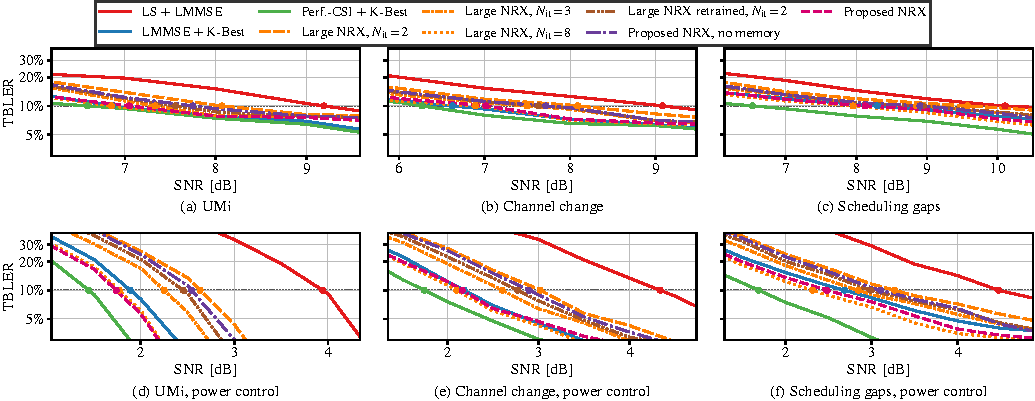
\includegraphics[width=\textwidth]{figures/tbler_vs_snr.pdf}
\caption{TBLER vs.\ SNR for $U\times B\equiv 2\times 4$ MU-MIMO and MCS index $i=14$ without power control, (a)--(c), and with power control, (d)--(f). Solid curves denote classical receivers and non-solid curves NRXs.}
\label{fig:tbler}
\end{figure*}

\subsection{Training}
We train the proposed NRX in two stages on simulated TB sequences rather than independent slots. Sequences of 8 to 64 slots use 3GPP tapped delay line (TDL), urban microcell (UMi), and urban macrocell (UMa) channels~\cite{tr38901} with Doppler shifts up to 400\,Hz. They include near-far UEs, as well as scheduling gaps and channel changes, which expose the receiver to missing and outdated memory entries. In the first stage, we retrain the Large NRX with $N_{\mathrm{it}}=2$, starting from its released weights~\cite{wiesmayr2025realtime}. In the second stage, we add the pilot memory and the channel filter to this retrained NRX and continue to train its weights.

The loss of both stages is the binary cross-entropy of the LLRs with respect to the transmitted bits plus, weighted by 0.01 as in the Large NRX, the mean squared error of the auxiliary channel estimate. In the first stage, we also distill knowledge from the released Large NRX with $N_{\mathrm{it}}=8$: the cross-entropy is computed with equal weights with respect to the transmitted bits and to the bit probabilities of that NRX, which thus serves as a teacher~\cite{hinton2015distilling}. The second stage uses no teacher. We use the Adam optimizer~\cite{kingma2015} with a learning rate of $10^{-4}$ and 8 sequences per step, halve it when the TBLER on a separate validation dataset, checked every $10^{3}$ steps, has not improved for two checks, and select the checkpoint with the lowest validation TBLER, reached after $1.1\cdot 10^{4}$ and $6\cdot 10^{3}$ steps in the two stages.
